\chapter{Easy PEasy -{} Part 2.}

\section{Introduction.}
\label{ch26-intro}%hyperlabel{ch26-intro}%

At the end of the previous chapter -{} Easy PEasy\program{EasyPEasy} Part 1, I promised to take a look
        at the various code routines that George has written to make life a lot easier for
        PE assembly language programmers. If you haven't already done so, get over to
        George's web site and download the programs mentioned last time. The website
        address is \url{http://gwiltprogs.info/}.

\section{Easy PEasy.}
\label{ch26-easy-peasy}%hyperlabel{ch26-easy-peasy}%

As I mentioned last time, Easy PEasy\program{EasyPEasy} isn't a program you can run, it is a
        collection of information and small binary files that you can include with your
        own programs -{} using the LIB and IN commands in your source code and assembling
        with GWASL\program{Gwasl} -{} to make programming the Pointer
        Environment a little easier.

\section{Supplied Files.}
\label{ch26-files-supplied}%hyperlabel{ch26-files-supplied}%

With Easy PEasy\program{EasyPEasy}, there are a number of files supplied, these are:

{\bf Keys\_pe} 
A file that can be included in your source file to define a number of
            equates for the various Trap \#3 routines introduced by the PE.

{\bf Keys\_wdef} 
Another include file. This one defines the WMAN\program{WMAN} window definition
            equates.

{\bf Keys\_wman} 
Similar to keys\_pe above but this file defines the
            equates for WMAN\program{WMAN} routines and vectors.

{\bf Keys\_wstatus} 
This file defines the equates etc for the window status area.

{\bf Keys\_wwork} 
This file contains the definitions for the window working
            definition.

{\bf Qdos\_pt} 
The equates etc for the PE interface.

{\bf Csprc\_bin} 
Some sprites, mostly for mode 4 but a few exist for mode 8. This file
            should be LIBbed by your own programs to use the sprites.

{\bf Csprc\_sym\_lst} 
This file lists the names of all the sprites in the above file. If you
            need to use a sprite in the above (binary) file, you must use the name listed
            in this file.

{\bf Peas\_bin} 
This file contains all the useful code subroutines that George has
            written to make using the PE from assembly language easy. This file is binary
            and as such, should be LIBbed by your source code.

{\bf Peas\_sym\_lst} 
This file lists all the routines supplied in the above file. Make sure
            that you use the name(s) listed in this file if you wish to use George's code
            in your own PE programs.


\section{Subroutines in Easy PEasy.}
\label{ch26-sub-routines}%hyperlabel{ch26-sub-routines}%

The file peas\_bin should be included at the very end of your
        own program's code, as follows:

\begin{lstlisting}[firstnumber=1,caption={Invoking EasyPEasy in Your Own Programs}]
         in        win1_source_easypeasy_peas_sym_lst
         lib       win1_source_easypeasy_peas_bin
\end{lstlisting}

The first `in' line includes the peas\_sym\_lst file
        which defines offsets from the current position to the entry points for the
        routines in the peas\_bin file which is copied `as is'
        straight into your final executable file. For this reason, you must keep these
        lines together and in the order shown above.


\begin{table}[htbp]
\centering
\begin{tabular}{l p{0.8\textwidth}}
\toprule
\textbf{Routine} & \textbf{Description}  \\
\midrule
%
GetSp & Allocates an area of memory and returns the address in A0.L. The size of the area required must be passed in D1.L on entry. No other registers are affected. Exits via SUI (see below) if the memory allocation causes an error.\\
Rechp & Deallocates and frees an area of memory allocated by GetSp above. The address should be passed in A4.L. No other registers are affected.\\
Move & Processes a MOVE request then returns with D4 and D0 both set to zero. No other registers are affected. Can be called from inside the MOVE action routine in your own programs.\\
Sleep & Puts the program to sleep and creates a button in the button frame - if present. If the button frame is not present, the button will be placed on the top left of the display. See below for register usage.\\
Set\_AP & Set an application window menu. See below for register usage. All registers are preserved on exit.\\
Sui & The program exits without warning and without any error messages. GetSp above will exit through here if there is an error when allocating memory.\\
%
\bottomrule
\end{tabular}
\caption{EasyPEasy Library Routines}
\label{tab:EasyPEasyLibraryRoutines}
\end{table}

\subsection{GetSp}
\label{ch26-sub-getsp}%hyperlabel{ch26-sub-getsp}%

GetSp allocates an area of memory for the current job, and returns the
            address in register A0.L. There are no errors returned (in D0) as the routine
            exits through sui (below) if it detects an error. Only register A0.L is
            affected by the routine -{} all others are preserved.

On entry, the number of bytes required should be held in D1.L. On exit,
            A0.L holds the address of the allocated area. An example of use, taken from
            George's example EX0\_asm, can be see in \lstlistingname~\ref{lst:EasyPeasyGetSPExample}.

\begin{lstlisting}[firstnumber=1,caption={EasyPEasy - GetSP Example},label={lst:EasyPeasyGetSPExample}]
         ...
         move.l    #ww0_0,d1      ; Size of working definition.
         bsr       getsp          ; Return ALCHP'd address in A0.
         movea.l   a0,a4          ; Copy to A4.
         ...
\end{lstlisting}

There is no requirement to check for an error with this routine, if it
            returns to your program then it has worked.

\subsection{Rechp}
\label{ch26-sub-rechp}%hyperlabel{ch26-sub-rechp}%

Rechp returns an area of memory, probably allocated using GetSp above,
            to the system. The address to deallocate must be passed in A4.L. All other
            registers are preserved and no errors are returned by this routine. An example
            of use would be after unsetting a widow definition, as per the following from
 EX0\_asm:

\begin{lstlisting}[firstnumber=1,caption={EasyPEasy - Rechp Example},label={lst:EasyPeasyRechpExample}]
         ...
         jsr       wm_unset(a2)
         bsr       rechp
         ...
\end{lstlisting}

Again, there is no need to check for errors as the routine never
            fails.

\subsection{Move}
\label{ch26-sub-move}%hyperlabel{ch26-sub-move}%

Move is called when a program detects that the user has requested a MOVE
            be carried out. The routine can be called either from your own code (if the
            read pointer loop exits with D0/D4 not zero) or from within an action routine
            called by the read pointer loop. In either case, calling the move routine is
            as simple as this:

\begin{lstlisting}[firstnumber=1,caption={EasyPEasy - Move Example},label={lst:EasyPeasyMoveExample}]
; MOVE loose item action routine.         
afun0_0  bsr       move            ; Process a MOVE.
         ...
\end{lstlisting}

The above is another example taken from George's
 EX0\_asm example program. After processing the move, the
            program needs to reset the loose item that caused the move request. See below
            for a fuller explanation of the example program and the code that is used to
            reset the loose items.

\subsection{Sleep}
\label{ch26-sub-sleep}%hyperlabel{ch26-sub-sleep}%

Sleep sets the program to a button which contains the name of the
            program and is placed in the button frame if there is one or at the top left
            of the screen if there isn't.

While in button mode, A HIT -{} left mouse click or SPACE -{} on the button
            will cause the program to waken and restore itself to full size again.

A DO -{} right mouse click or ENTER -{} on the button will cause the program
            to waken if the program is currently located in the button frame, or, causes a
            move if the button frame is not present.

The registers required to call sleep are shown in \tablename~\ref{tab:EasyPEasySleepEntryRegisters}.

\begin{table}[htbp]
\centering
\begin{tabular}{l p{0.8\textwidth}}
\toprule
\textbf{Register} & \textbf{Description}  \\
\midrule
%
D1.L & The size needed for the button. Can be obtained from ww0\_1.\\
D2.L & The size needed for main window. Can be obtained from ww0\_0.\\
A2.L & The WMAN vector.\\
A4.L & Pointer to the window working definition for the button window.\\
%
\bottomrule
\end{tabular}
\caption{EasyPEasy Sleep Entry Registers}
\label{tab:EasyPEasySleepEntryRegisters}
\end{table}


On exit from the sleep routine, the registers are set as per \tablename~\ref{tab:EasyPEasySleepExitRegisters}.

\begin{table}[htbp]
\centering
\begin{tabular}{l p{0.8\textwidth}}
\toprule
\textbf{Register} & \textbf{Description}  \\
\midrule
%
D1-D3 & Undefined. \\
A0.L  & The channel ID.\\
A1.L  & Undefined.\\
A2.L  & Preserved - the WMAN vector.\\
A3.L  & The window definition address.\\
A4.L  & Pointer to the working definition which may have changed.\\
%
\bottomrule
\end{tabular}
\caption{EasyPEasy Sleep Exit Registers}
\label{tab:EasyPEasySleepExitRegisters}
\end{table}


As before, the following is an example from EX0\_asm             where the SLEEP loose item sets the sleep event in D4 and returns. This causes
            the read pointer loop to exit back to the user's code where the events etc are
            checked. The following extract shows the checks made to handle the sleep event
            being detected:

\begin{lstlisting}[firstnumber=1,caption={EasyPEasy - Sleep Example},label={lst:EasyPeasySleepExample}]
         ...
no_er2   btst      #pt__zzzz,wsp_weve(a1) ; Was it a SLEEP event?
         beq.s     wrpt            ; No, read the pointer again
         move.l    #ww0_1,d1       ; Get main window button size
         move.l    #ww0_0,d2       ; Get main window size
         bsr       sleep           ; Process a SLEEP
         bra.s     wrpt            ; Read the pointer again
         ...
\end{lstlisting}

In the above extract, we can see D1 and D2 being set to the sizes
            calculated (by SETW\program{SETW} -{} see previous chapter) for the main window and the
            buttonised window. Registers A2 and A4 are correctly set.

After calling sleep, the program must continue to read the pointer
            otherwise it won't know if a DO or a HIT has been detected, or if it has been
            woken from slumber etc.

\subsection{Set\_AP}
\label{ch26-sub-set_ap}%hyperlabel{ch26-sub-set_ap}%

Set\_AP is used to create an application window menu within a particular
            application window for a program. It is assumed that each item in the menu
            will be exactly the same length, although if QDOS strings are being used the
            word count for each one will determine what appears.

The registers required to call Set\_AP are defined in \tablename~\ref{tab:EasyPEasySetAPEntryRegisters}.

\begin{table}[htbp]
\centering
\begin{tabular}{l p{0.8\textwidth}}
\toprule
\textbf{Register} & \textbf{Description}  \\
\midrule
%
D1.W & How many items are present?\\
D2.W & The length of each item.\\
A0.L & Pointer to the start of the list of items.\\
A1.L & Pointer to the application window.\\
A4.L & Pointer to the window working definition.\\
%
\bottomrule
\end{tabular}
\caption{EasyPEasy Set\_AP Entry Registers}
\label{tab:EasyPEasySetAPEntryRegisters}
\end{table}

On exit, all registers are preserved.

George has provided an example program that uses this routine,
 EX1\_asm. When run, the program displays a list of files
            on flp1\_ when you click on the Display loose item. You can then select as many
            files as you wish, and click the Copy loose item. The selected files will then
            be copied to ram1\_. The appropriate extract from this demonstration program
            is:

\begin{lstlisting}[firstnumber=1,caption={EasyPEasy - SetAP Example},label={lst:EasyPeasySetAPExample}]
         ...
         movea.l   fnmes(a6),a0    ; Pointer to list of file names
         moveq     #36,d2          ; Interval between entries
         movea.l   a1,a5           ; Needed later on, saved
         movea.l   ww_pappl(a4),a1 ; List of app window pointers
         movea.l   (a1),a1         ; Get app window 0 from list
         bsr       set_ap          ; Set the app window menu
         ...
\end{lstlisting}

The program has previously read the directory of all files (but no
            directories etc) on flp1\_ into the area of memory addressed by A0. The data
            stored there (effectively) looks like the following:

\begin{lstlisting}[firstnumber=1,caption={EasyPEasy - SetAP Item List},label={lst:EasyPeasySetAPItemList}]
         ...
item_1   dc.w      4               ; Length of string
         dc.b      'boot'          ; Filename from flp1_
         dc.b      0,0, ...        ; 32 padding bytes

item_2   dc.w      7               ; Length of string
         dc.b      'boot_pe'       ; Filename from flp1_
         dc.b      0,0, ...        ; 29 padding bytes
         ...
\end{lstlisting}

You can see from the above that each entry is a total of 36 bytes long
            (the difference between addresses item\_1 and item\_2) although the actual menu
            items themselves, the filename, need not be exactly 36 bytes. Regardless of
            the value of the padding bytes, the data displayed in the menu items will only
            show the actual filenames as defined by the QDOS strings making up each
            item.

An article of application window menus will be coming soon in this
            series.

\subsection{Sui}
\label{ch26-sub-sui}%hyperlabel{ch26-sub-sui}%

Sui is a dramatic routine to call. Wherever your program is in its
            processing, calling sui will cause it to exit. In addition, the GetSp routine
            (above) will call sui if it cannot allocate a suitable area of memory.
            George's example program calls sui when it detects that the Pointer
            Environment is not present, as follows:

\begin{lstlisting}[firstnumber=1,caption={EasyPEasy - Sui Example},label={lst:EasyPeasySuiExample}]
         ...
         moveq     #iop_pinf,d0    ; Find Pointer Environment & WMAN
         moveq     #-1,d3          ; Timeout
         trap      #3              ; Do it
         tst.l     d0              ; Did it work?
         bne       sui             ; Failed, or PE absent, bale out
         ...
\end{lstlisting}

No registers are used by this routine. It never returns an error -{}
            because it never actually returns!

\section{The Example Program, EX0\_asm.}
\label{ch26-ex0}%hyperlabel{ch26-ex0}%

So, having discussed the various bits and pieces of Easy PEasy\program{EasyPEasy}, lets dissect
        one of George's example. The simplest example is EX0\_asm and
        its corresponding SETW\program{SETW} designed window file,
 EX0w\_asm, so those are what we will look at next.

This example simply shows how to use the four main events in a PE
        program:
\begin{itemize}[itemsep=0pt]

\item{}Move -{} moves the window around the screen.


\item{}Resize -{} allows the window to be sized.


\item{}Sleep -{} puts the program to sleep either in the button frame, if
                present, or on screen.


\item{}Esc -{} exit from the program.

\end{itemize}

The program looks like Figure~\ref{fig:ExampleProgramEX0InAction} when running on QPC:

\begin{figure}[h]
\center
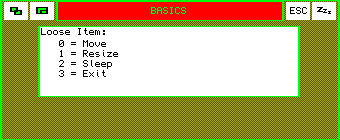
\includegraphics[width=0.75\textwidth,keepaspectratio=true]{Content/images/peas_ex0.png}
\label{fig:ExampleProgramEX0InAction}
\caption{Example program EX0 in action.}
\end{figure}


The window in Figure~\ref{fig:ExampleProgramEX0InAction} shows an outline with a green border and an
 \emph{interesting} paper colour. A white information window is
        displayed listing the various loose items in the program. The information window
        is white with a green border and black ink.

Along the very top of the window we can see the program's title -{} BASICS -{}
        in a red papered information window with a green border and ink, and the four
        loose items for MOVE and SIZE on the left with ESC and SLEEP on the right.

The window has been created by SETW\program{SETW} and the definitions are all held in the
        file EX0w\_asm which is supplied in the
 peass download from George's web site.

What follows is a slightly amended version of the program supplied by
        George. I have updated some of the comments to make then more readable and
        understandable (by me!) and in a couple of places, I have rearranged the order of
        some of the instructions -{} with George's blessings of course.

\begin{lstlisting}[firstnumber=1,caption={Ex0 - Standard Job Header}]
;----------------------------------------------------------------------
; Standard job header.
;----------------------------------------------------------------------
         bra.s     start
         dc.l      0
         dc.w      $4afb

fname    dc.w      fname_e-fname-2
         dc.b      "EX0 v1.05"
fname_e  ds.b      0
         ds.w      0

;----------------------------------------------------------------------
; Include the various Easy PEasy include files. These give us names for
; all the various offsets, vectors, traps etc used by the PE.
;----------------------------------------------------------------------
         in        win1_ass_pe_keys_pe
         in        win1_ass_pe_qdos_pt
         in        win1_ass_pe_keys_wwork
         in        win1_ass_pe_keys_wstatus
         in        win1_ass_pe_keys_wman
         in        win1_ass_pe_keys_wdef


;----------------------------------------------------------------------
; Define a few explicit equates for this example program. These are 
; offsets into the program's dataspace (relative to A6) where we store
; various bits of useful information, channel ids and so on.
;----------------------------------------------------------------------
id       equ       0
wmvec    equ       4
slimit   equ       8               ; Size - origin
\end{lstlisting}

The above is the usual QDOSMSQ job header, and so on. The various
 IN lines pull in the include files from Easy PEasy\program{EasyPEasy}.

\begin{lstlisting}[firstnumber=last,caption={Ex0 - Initialisation}]
;----------------------------------------------------------------------
; Here is when the example code really starts.
;----------------------------------------------------------------------
start    lea       (a6,a4.l),a6    ; Dataspace in A6
         bsr.s     ope             ; Open a con channel
         move.l    a0,id(a6)       ; Keep the ID safe
         moveq     #iop_pinf,d0    ; Find Pointer Environment & WMAN
         moveq     #-1,d3          ; Timeout
         trap      #3              ; Do it
         tst.l     d0              ; Did it work?
         bne       sui             ; Failed, or PE absent, bale out
         move.l    a1,wmvec(a6)    ; Keep WMAN vector safe too
         beq       sui             ; WMAN not present, bale out
         movea.l   a1,a2           ; Copy WMAN vector to A2
         lea       slimit(a6),a1   ; Buffer for results
         moveq     #iop_flim,d0    ; Find maximum size of window
         trap      #3              ; Do it
         subi.l    #$C0008,(a1)    ; Less 12, 8 from width, height
         lea       wd0,a3          ; Address of main window definition
         move.l    #ww0_0,d1       ; Size of working definition
         bsr       getsp           ; Return ALCHP'd address in A0
         movea.l   a0,a4           ; Copy to A4.
\end{lstlisting}

The section of code above carries out various initialisations and checks for
        the Pointer Environment and WMAN\program{WMAN} before allocating enough space for the working
        definition for the main window which SETW\program{SETW} stores for us
        in ww0\_0.

\begin{lstlisting}[firstnumber=last,caption={Ex0 - Loose Item Initialisation}]
;----------------------------------------------------------------------
; We need to set the status area to zeros
; and the loose items to "available" (zero).
;----------------------------------------------------------------------
         lea       wst0,a1         ; Status area address
         movea.l   a1,a0           ; Copy to A0
         moveq     #wst0_e-wst0-1,d1 ; Bytes to clear - 1

st1      clr.b     (a0)+           ; Set status to zero/available
         dbra      d1,st1          ; And repeat

         movea.l   id(a6),a0       ; Get the channel ID again
         move.l    wd_xmin+wd_rbase(a3),d1 ; Minimum size (x,y) in D1
         andi.l    #$0FFF0FFF,d1   ; Lop off the scaling factors
;                                  ; Wm_setup gets upset if you leave
;                                  ; scaling stuff attached. The x,y 
;                                  ; sizes in D1 must be actual sizes.
         jsr       wm_setup(a2)    ; Set up the working definition
\end{lstlisting}

Just before we (finally) set up the window, we need to be sure that all the
        loose items are set to available -{} in this case -{} and that the status area is
        filled with zeros. As ever, SETW\program{SETW} has put the status
        area details in an easy to find location -{} wst0 -{} and we use this to initialise
        the status area easily. Regardless of the actual size of the status area itself,
        the above code will always work.

Please note, in the above George picks the smallest window definition as the
        one to use when the program first starts. The size of the smallest definition is
        obtained from wd\_xmin + wd\_rbase(a3) and placed in D1.L with the high word
        containing the width and the low word holding the height. Because this definition
        has scaling details embedded in the top nibble of each word, these must be masked
        out before calling \pe{WM\_SETUP}.

The same applies if you set D1.L to zero -{} which means \emph{use the
        default (largest) definition} -{} unless the scaling factors are masked
        off, the call to \pe{WM\_SETUP} will return, but your window will not display correctly,
        if at all. This problem also affects the \pe{WM\_FSIZE} routine which returns the size,
        in D1.L, for a given definition. You \emph{must} mask off the
        scaling nibbles.

\begin{lstlisting}[firstnumber=last,caption={Ex0 - Position and Draw Window}]
         moveq     #-1,d1          ; Set the window position ...
         jsr       wm_prpos(a2)    ; ... to where the pointer is
         jsr       wm_wdraw(a2)    ; Draw the contents
\end{lstlisting}

The snippet of code above sets the window position to be where the pointer
        is on screen right now, then draws the window.

\begin{lstlisting}[firstnumber=last,caption={Ex0 - Reading the Pointer}]
wrpt     jsr       wm_rptr(a2)     ; Read the pointer
\end{lstlisting}

The above starts the pointer reading loop. This code will not return unless
        an action routine sets D0 with an error code, or, sets D4 with an event
        number.

\begin{lstlisting}[firstnumber=last,caption={Ex0 - Test for Errors or Events}]
         beq.s     no_err          ; As D0 is zero, D4 must be non zero
         bra       sui             ; Error, D0 is non zero, bale out
\end{lstlisting}

If we have returned from the read pointer loop, then D0 is holding an error
        code, or D4 holds an event number. Because the Status Register must hold the flags
        according to the value in D0 on exit from an action routine, checking for the Z
        flag being set implies that D0 is indeed holding an error.

If no error is detected, the code skips off to a label no\_err below, where
        D4 is checked for events to process, otherwise, the program dies horribly with a
        call to the sui routine supplied by George.

\begin{lstlisting}[firstnumber=last,caption={Ex0 - Console Channel Details \& Code}]
;----------------------------------------------------------------------
; Default console channel definition.
;----------------------------------------------------------------------
con      dc.w      3
         dc.b      'con'

;----------------------------------------------------------------------
; Routine to open a channel for this job.
;----------------------------------------------------------------------
ope      lea       con,a0          ; To open "con"
         moveq     #-1,d1          ; For this job
         moveq     #0,d3
         moveq     #io_open,d0
         trap      #2
         rts
\end{lstlisting}

The code above defines a console channel for our program and opens
        it.

\begin{lstlisting}[firstnumber=last,caption={Ex0 - Checking Events}]
no_err   movea.l   (a4),a1         ; Status area
         btst      #pt__can,wsp_weve(a1) ;Was it a CANCEL event?
         bne       sui             ; Yes, exit

         btst      #pt__move,wsp_weve(a1) ; Was it a MOVE event?
         beq.s     no_er1          ; No, skip
         bsr       move            ; Yes, process a MOVE
         bra.s     wrpt            ; Read pointer again

no_er1   btst      #pt__wsiz,wsp_weve(a1) ; Was it a SIZE event?
         beq       no_er2          ; No, skip
         bsr.s     resze           ; Yes, process a SIZE
         bra.s     wrpt            ; Read pointer again

no_er2   btst      #pt__zzzz,wsp_weve(a1) ; Was it a SLEEP event?
         beq.s     wrpt            ; No, read the pointer again
         move.l    #ww0_1,d1       ; Get main window button size
         move.l    #ww0_0,d2       ; Get main window size
         bsr       sleep           ; Process a SLEEP
         bra.s     wrpt            ; Read pointer again
\end{lstlisting}

The code above is executed on return from the read pointer loop with an
        event number in D4. It begins by checking to see if the CANCEL event occurred (or
        was set in an action routine) and if so, exits the program via the sui
        routine.

Assuming that the event was not CANCEL, the next check is for a MOVE event.
        If it was a MOVE, the move is handled by George's move routine and we return to
        the read pointer loop again.

The next check is for a SIZE event and if detected, we process the MOVE
        request and return to the pointer reading loop, otherwise we skip to the final
        check.

The last check we make is for a SLEEP event. If this is not a SLEEP request,
        we skip back and begin reading the pointer again. It this is a SLEEP request, we
        set the registers as required by the sleep routine by loading D1 with the current
        window size and D2 with the button window size -{} both helpfully defined by
 SETW -{} and jump into the sleep routine.

The sleep routine returns control to our code again and we skip back to
        reading the pointer. We must do this or we will never be able to know when the
        sleeping program has been wakened etc.

All of the above checks were made by looking at the individual bits in the
        window byte of the event vector.

\begin{lstlisting}[firstnumber=last,caption={Ex0 - Move Loose Item Action Routine}]
;----------------------------------------------------------------------
; Loose item action routines.
;----------------------------------------------------------------------
; MOVE
;----------------------------------------------------------------------
afun0_0  bsr       move            ; Process a MOVE

af1      move.w    wwl_item(a3),d1 ; Loose item number
         move.b    #wsi_mkav,ws_litem(a1,d1.w) ; Ask for redraw
         moveq     #-1,d3          ; Selective redraw
         jsr       wm_ldraw(a2)    ; Redraw loose items
         clr.b     ws_litem(a1,d1.w) ; Available status
         moveq     #0,d4           ; No events
         moveq     #0,d0           ; No errors
         rts                       ; Read the pointer again
\end{lstlisting}

The program demonstrates both methods of handling loose item action
        routines. MOVE and SIZE are handled within the read pointer loop and not by the
        above code which checks the event bits outside of the read pointer loop.

The action routine above, for a MOVE, carries out all the processing
        necessary to make the window move on screen. It simply calls the move routine
        supplied by George.

The code at label af1 is necessary as it resets the loose item's status to
        available -{} when a loose item is hit or done, its status changes to selected.
        Once this has been done and the loose item redrawn, D4 and D0 are set to tell the
        read pointer loop to continue, the action has been processed.

\begin{lstlisting}[firstnumber=last,caption={Ex0 - SIZE Loose Item Action Routine}]
;----------------------------------------------------------------------
; RESIZE
;----------------------------------------------------------------------                                    
afun0_1  move.l    a3,-(a7)        ; Save working register
         movea.l   ww_wdef(a4),a3  ; Window definition x,y size
         bsr.s     resze           ; Process a SIZE
         movea.l   (a7)+,a3        ; Restore pointer to loose item
         bra.s     af1             ; And reset status etc
\end{lstlisting}

The action routine above processes a SIZE request when the Size Loose Item
        is hit or done. It does this by calling code common to the action routine itself
        and called by the user level code (outside the pointer reading loop) when a SIZE
        event bit is set in the window event vector.

Unfortunately, there is no Easy PEasy\program{EasyPEasy} way to do a resize (at least, not at
        the moment) so we programmers have to do it all ourselves. As shown below.

\begin{lstlisting}[firstnumber=last,caption={Ex0 - SIZE Processing}]
;----------------------------------------------------------------------
*  To perform the resize we need to
*    a. Find the amount of resize (by wm_chwin)
*    b. Throw away the current working definition (by wm_unset)
*    c. Find the new size (by wm_fsize)
*    d. Get space for the new working definition (by getsp)
*    e. Set up the new working definition  (by wm_setup)
*    f. Position the new window  (by wm_prpos)
*    g. Draw the contents  (by wm_wdraw)
*
* Comments
*   On a.
*    We have to set the resize bit in the window byte of the
*    event vector in the status area before wm_chwin is called.
*    The change in size is returned in D1 and the window size
*    event number is returned in D4.
*
*   On c.
*    On entry to wm_fsize, D1 must contain the requested size.
*    This size must be chosen carefully. It must be no bigger
*    than the maximum in the window definition. It must be
*    smaller than the maximum size for the window layout. The
*    x-size must be a multiple of 4 (to allow proper stippling.
*    Finally the size must not be bigger than the current screen
*    size with allowance for shadow and border.
*    On exit D1 contains the actual size and D2.W contains the
*    number of the repeated section.
*    In this example we do not really need to use wm_fsize since
*    we know that D2.W will be zero and that the value in D1
*    will be that on entry (since we have a variable window).
*
*   On d.
*    The space needed is found from the label ww0_0 set in the
*    window definition.
*
*   On e.
*    For wm_setup we need on entry:
*     D1 = size
*     A0 = channel ID
*     A1 -> status area
*     A3 -> window definition
*     A4 -> space for working definition
*
*   On f.
*    On entry to wm_prpos we need the position in D1.
*    In order to ensure that the bottom right corner of the
*    resized window is in the same position as that of the old
*    we need to subtract the increase in size from the pointer
*    origin in the old window.
*    The new position is thus wd_org plus ww_xsize minus the
*    new size.
*
;----------------------------------------------------------------------   
resze    move.l    ww_xorg(a4),d7
         move.l    ww_wdef(a4),a5           Window def
         add.l     wd_xorg(a5),d7
         add.l     ww_xsize(a4),d7          Ptr pos for PRPOS (optr)
         bset      #pt__wsiz,wsp_weve(a1)
         jsr       wm_chwin(a2)             Sets change to D1 (mv)
         bclr      #pt__wsiz,wsp_weve(a1)
         move.w    wd_rbase+wd_xmin(a5),d5
         andi.w    #$fff,d5
         move.w    ww_xsize(a4),d4
         swap      d1
         sub.w     d1,d4
         cmp.w     d5,d4
         bgt.s     resze1                   D4 is greater
         move.w    d5,d4

resze1   move.w    wd_xsize(a5),d5
         cmp.w     d5,d4
         blt.s     resze2                   D4 is smaller
         move.w    d5,d4

resze2   moveq     #3,d3
         add.w     d4,d3
         andi.w    #$fffc,d3                Keep answer in D3.W  (mv)
         move.w    wd_rbase+wd_ymin(a5),d5
         andi.w    #$fff,d5
         move.w    ww_ysize(a4),d4
         swap      d1
         sub.w     d1,d4
         cmp.w     d5,d4
         bgt.s     resze3                   D4 is greater
         move.w    d5,d4

resze3   move.w    wd_ysize(a5),d5
         cmp.w     d5,d4
         blt.s     resze4                   D4 is smaller
         move.w    d5,d4

resze4   swap      d3
         move.w    d4,d3                    D3 = new mv x | y
         jsr       wm_unset(a2)
         bsr       rechp

;----------------------------------------------------------------------
; Now restrict size to the screen size less (12,8)
;----------------------------------------------------------------------
         move.l    slimit(a6),d1
         cmp.w     d3,d1
         ble       resze7                   D1 OK
         move.w    d3,d1

resze7   swap      d1
         swap      d3
         cmp.w     d3,d1
         ble       Resze8                   D1 OK
         move.w    d3,d1                    New size

resze8   swap      d1                       New limited size
         move.l    d1,d3
         jsr       wm_fsize(a2)
         move.l    d1,-(a7)                 Keep size pro tem
         move.l    #ww0_0,d1                Space needed
         bsr       getsp
         move.l    (a7)+,d1                 Replace size
         movea.l   a0,a4                    New wwd
         movea.l   id(a6),a0                Replace ID
         jsr       wm_setup(a2)

;----------------------------------------------------------------------
; The position for PRPOS is optr-mv with minimum of 4 | 2
;----------------------------------------------------------------------
         move.l    d7,d1
         swap      d1
         swap      d3
         sub.w     d3,d1
         cmpi.w    #4,d1
         bge.s     resze5                   D1 not less than 4
         move.w    #4,d1                    Set minimum of 4

resze5   swap      d1
         swap      d3
         sub.w     d3,d1
         cmpi.w    #2,d1
         bge.s     resze6                   D1 not less than 2
         move.w    #2,d1                    Set minimum of 2

resze6   jsr       wm_prpos(a2)
         jmp       wm_wdraw(a2)
\end{lstlisting}

The above code is George's way of processing a SIZE request from within an
        action routine or from user code that detected the SIZE bit set in the window
        event vector.

The other two action routines, for SLEEP and ESC, demonstrate how an action
        routine can simply set the appropriate bit in the window vector, set D4 to
        indicate an event and exit with D0 cleared.

In this case, the actions cause the pointer reading loop to return to the
        user's code where the events can be checked for (see above) and processed
        accordingly.

\begin{lstlisting}[firstnumber=last,caption={Ex0 - EXIT Loose Item Action Routine}]
;----------------------------------------------------------------------
; EXIT - set the CANCEL event in the windows event vector, put the 
; CANCEL event number in D4 and exit with D0 set to zero.
;----------------------------------------------------------------------
afun0_3  bset      #pt__can,wsp_weve(a1) ; Set CANCEL window event
         moveq     #pt__can,d4     ; ESC event number
         moveq     #0,d0           ; No errors
         rts                       ; Return to exit from reading the 
;                                  ; pointer and into the PROCESS EVENT 
;                                  ; section of the user's code.
\end{lstlisting}

First of all, the action routine for the ESC loose item. This is the
        simplest action routine as it only has to set the event bit, set D4 and D0 then
        exit. It doesn't have to reset the ESC loose item status from selected back to
        available because the program is about to exit and the user will never see the
        redrawn loose item. Simple.

\begin{lstlisting}[firstnumber=last,caption={Ex0 - SLEEP Loose Item Action Routine}]
;----------------------------------------------------------------------
; SLEEP - set the ZZZ event bit in the window event vector, put the ZZZ
; event number in D4, redraw the ZZZ loose item as available - else it
; is still selected when we wake from the button frame - then exit with
; D0 set to zero.
;----------------------------------------------------------------------
afun0_2  move.w    wwl_item(a3),d1 ; Item number for the ZZZ loose item
         move.b    #wsi_mkav,ws_litem(a1,d1.w) ; Redraw as available
         moveq     #-1,d3          ; Selective redraw
         jsr       wm_ldraw(a2)    ; Redraw loose items
         clr.b     ws_litem(a1,d1.w) ; Available status set
         bset      #pt__zzzz,wsp_weve(a1) ; Set ZZZ window event.
         moveq     #pt__zzzz,d4    ; ZZZ event number
         moveq     #0,d0           ; No errors
         rts                       ; Return to exit from reading the 
;                                  ; pointer and into the PROCESS EVENT 
;                                  ; section of the user's code.
\end{lstlisting}

The sleep loose item's action routine is almost as simple, but because the
        program will -{} hopefully -{} be awakened at some point, it has to reset the loose
        item status and redraw it.

The code above starts off by obtaining the correct loose item number and
        changing its status to indicate that it is available. It then calls \pe{WM\_LDRAW} to
        redraw only those loose items asking for a status change \& redraw -{} as
        signalled by the value of minus one in D3. This prevents redrawing up to 32 loose
        items which don't need redrawing because nothing has changed.

Once redrawn, the loose item's status is set to available as well, the SLEEP
        bit is set in the window event vector, D4 is set to show the event number and we
        exit with D0 cleared to show that no errors occurred.

On return from the above two action routines, the read pointer loop will
        exit and processing will continue from the \lstinline{beq.s no_err} just after the wrpt
        label. (Many lines above!)

% lstinline resets the "last" listing line number. Damn!
\begin{lstlisting}[firstnumber=305,caption={Ex0 - Includes and Libraries}]
;----------------------------------------------------------------------
; Pull in window definition as created by SETW.
;----------------------------------------------------------------------
         in        win1_ass_pe_EX0w_asm

;----------------------------------------------------------------------
; Pull in the Easy PEasy stuff next - code routines and sprites.
;----------------------------------------------------------------------
         in        win1_ass_pe_peas_sym_lst
         lib       win1_ass_pe_peas_bin

         in        win1_ass_pe_csprc_sym_lst
         lib       win1_ass_pe_csprc_bin
\end{lstlisting}

The last few lines of code pull in the SETW\program{SETW} defined window from the file
        EX0w\_asm, then LIBs in the Easy PEasy\program{EasyPEasy} routines and the various sprites that your
        program might want to use.

\section{Coming Up...}

The next chapter in the ongoing saga of writing PE
        programs in assembler, will concentrate on application windows and their
        window menus.

